\chapter{Basic genetic circuits in steady state - The master equation}
\label{ch:master}

In this chapter, we develop a model of a genetic system considering only its intrinsic noise using the master equation, which is an approach to model stochastic processes where there are defined states and there are certain transition probabilities between states.

This chapter is based on the work done by M. Thattai and A. van Oudenaarden in \cite{thattai01}.

\section{Single gene}

For the process of transcription and translation the number $d$ of DNA copies of certain gene is taken to be constant and the rate $k_r$ of production of RNA ($n_1$) is proportional to $d$. In the same way, the rate $k_p$ of production of proteins ($n_2$) per mRNA is constant. There is also a degradation rate for each molecule proportional to their concentration. The model is ilustrated in fig. \ref{fig:mas-dogma}.

\begin{figure}[H]
  \centering
  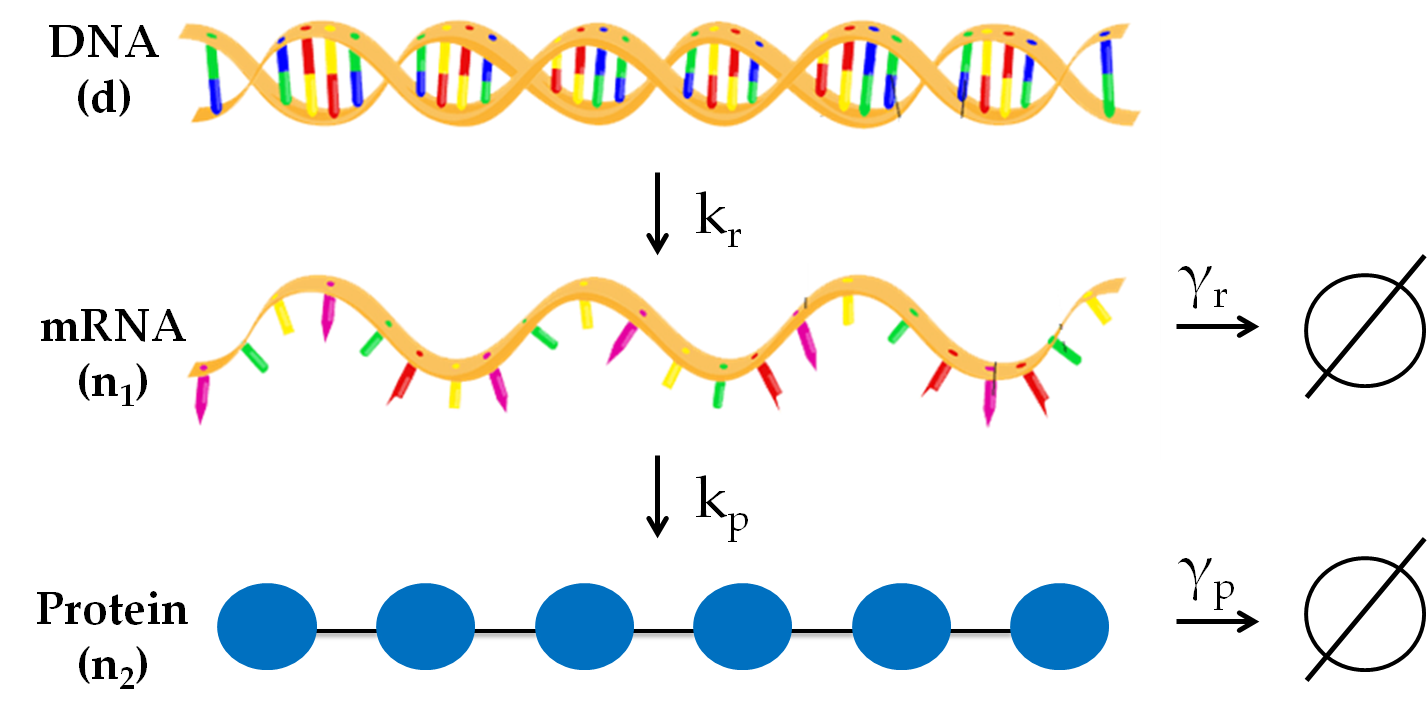
\includegraphics[width=8cm]{mas-dogma}
  \caption[Model of gene expression for a single gene]{\label{fig:mas-dogma} Steps of gene expression considered in the model. Taken from \cite{thattai01}.}
\end{figure}

The deterministic equations describing these processes are therefore given by

\begin{align}
  \dot{n_1}(t) &= k_rd-\gamma_rn_1(t)\label{eq:mas-simple_det_1},\\
  \dot{n_2}(t) &= k_pn_1(t)-\gamma_pn_2(t) \label{eq:mas-simple_det_2}.
\end{align}

Hence, on steady state

\begin{align}
  \langle n_1 \rangle_s &= \frac{k_r}{\gamma_r} \label{eq:mas-simple_ss_1}, \\
  \langle n_2 \rangle_s &= \frac{k_p}{\gamma_p} \langle n_1 \rangle_s = \frac{k_pk_r}{\gamma_p\gamma_r} \label{eq:mas-simple_ss_2}.
\end{align}

But these are numbers of molecules which are discrete, and on that discreteness lies part of the stochastic behaviour of those kind of systems. The molecules are created and degradated one at a time at a certain average rate but the timing between each creation or degradation should not match exactly the rates. 

To model the intrinsic noise, we will consider each pair of values of $(n_1,n_2)$ as a possible state for the system. There are transitions between the possible states which are proportional to the rates of creation and degradation as can be seen on figure \ref{fig:mas-trans_single}.

\begin{figure}[H]
  \centering
  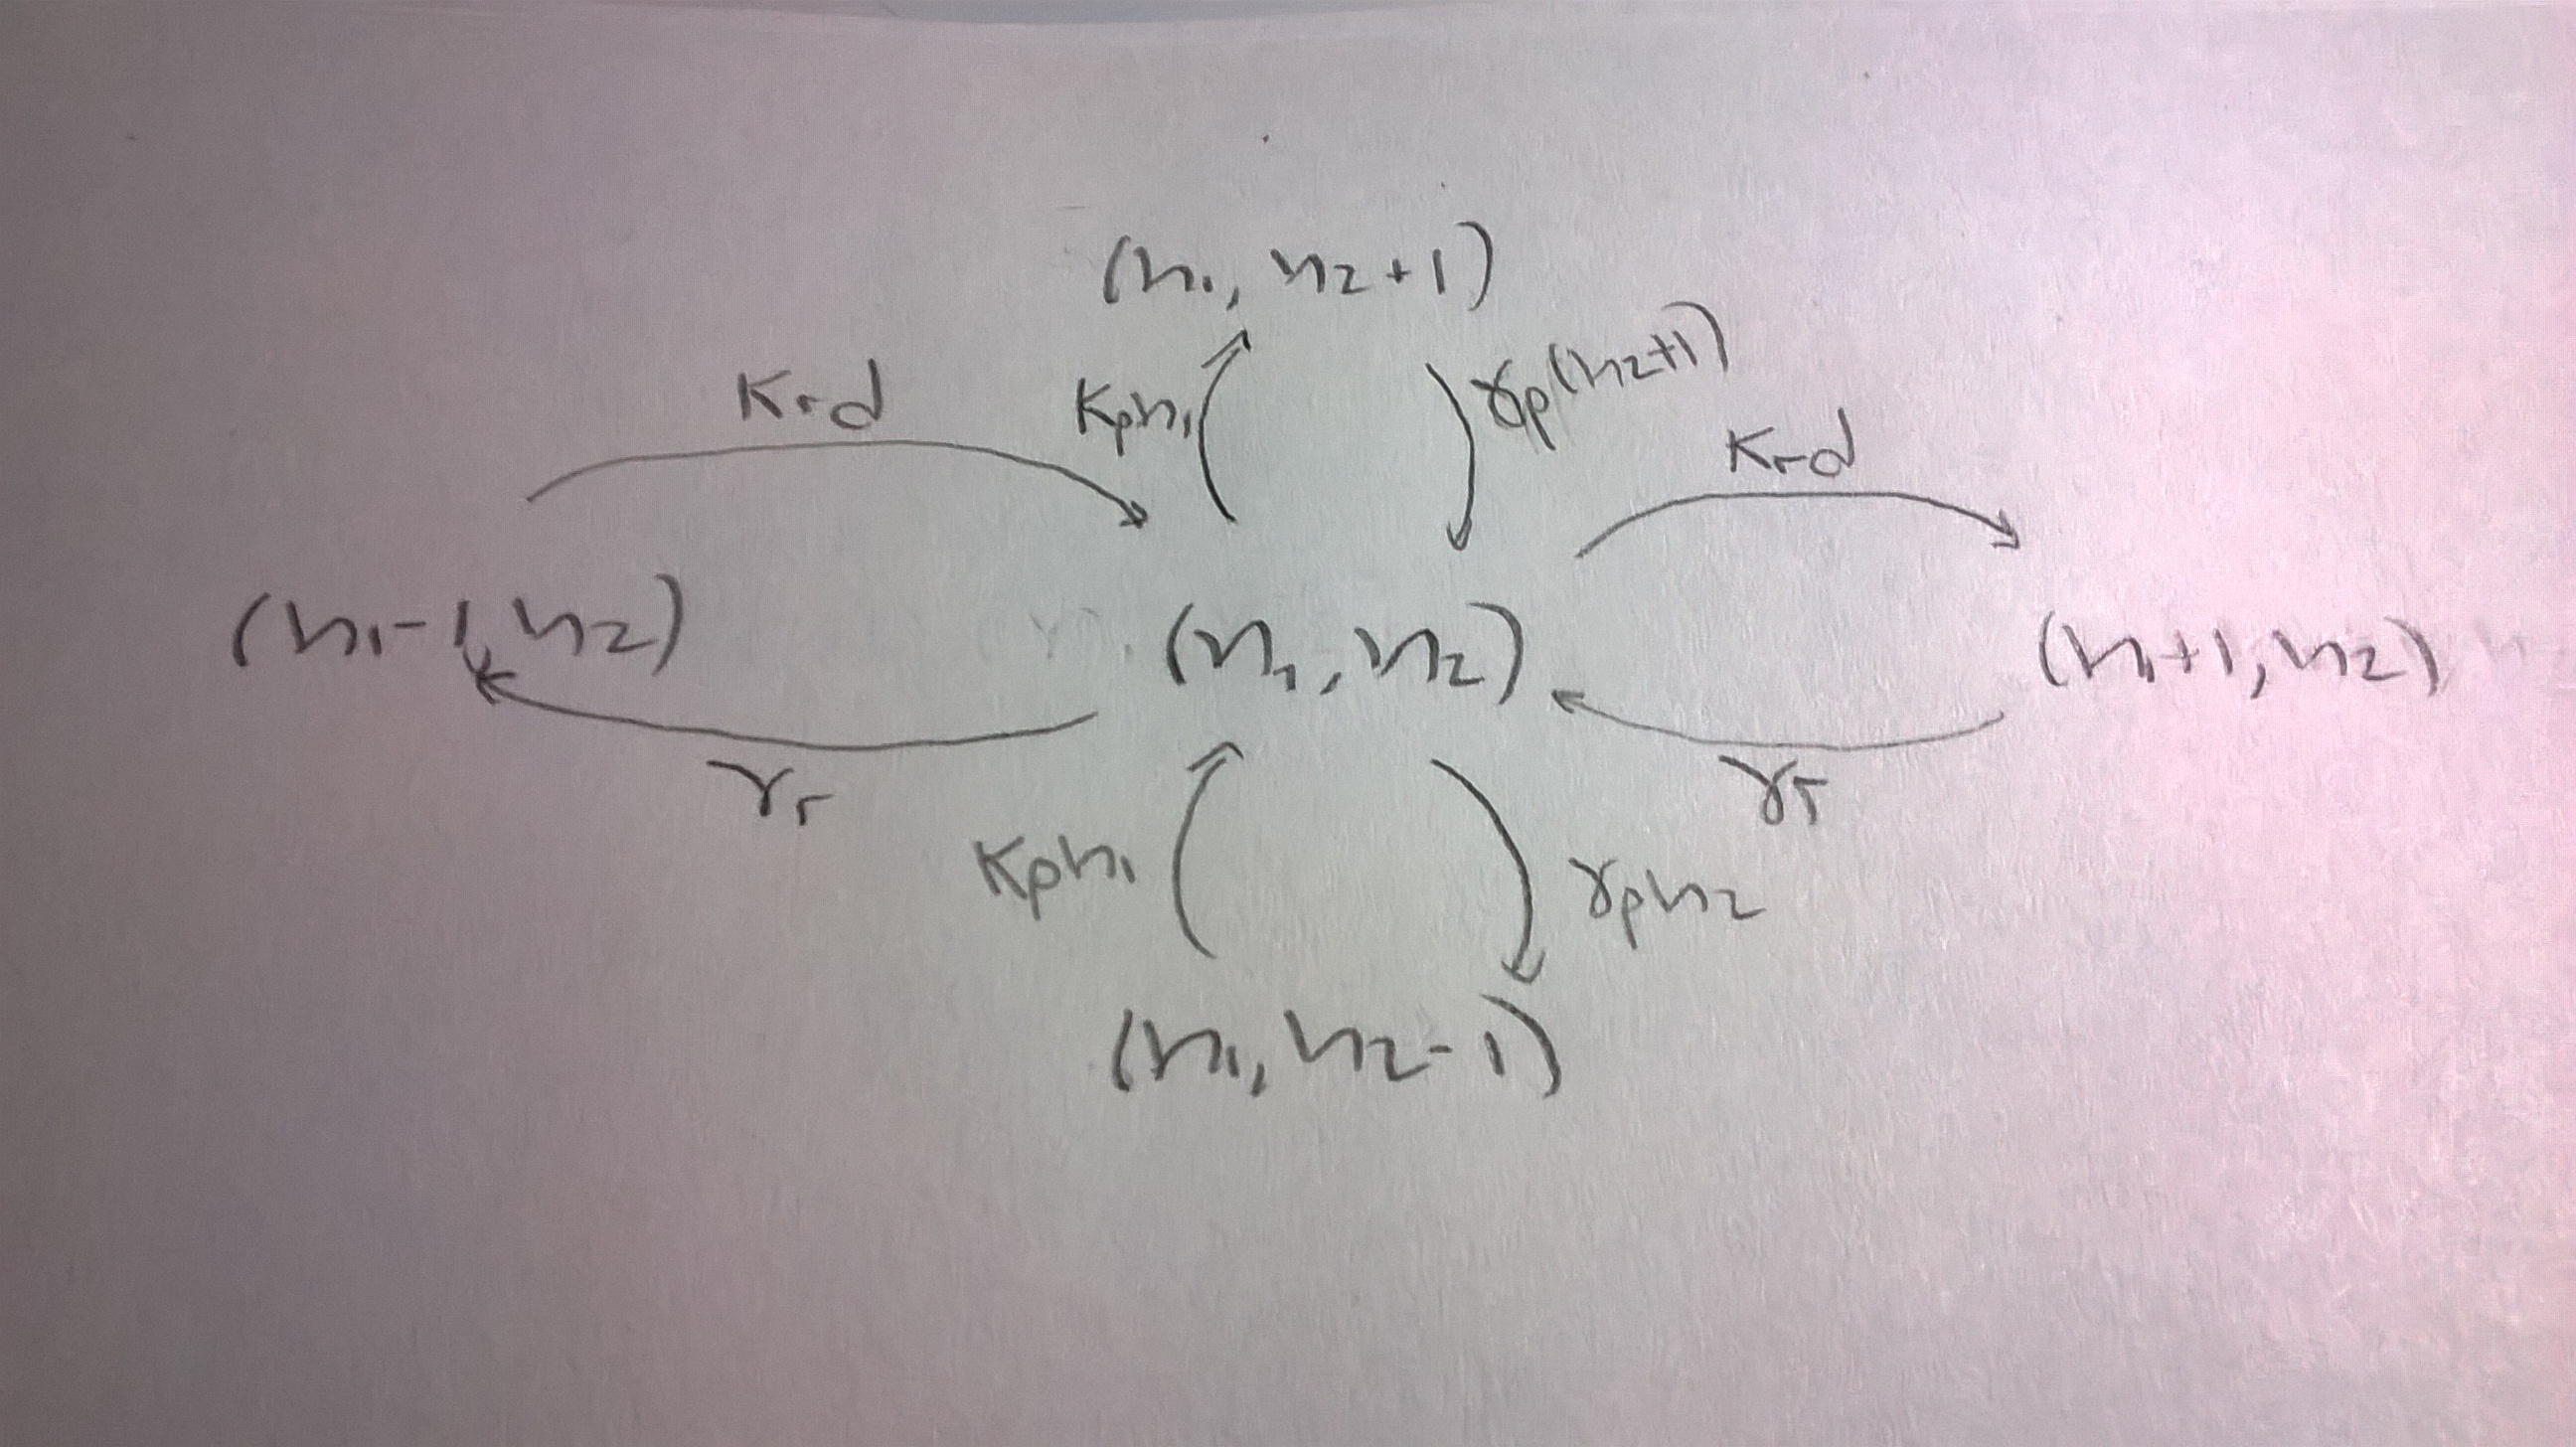
\includegraphics[width=8cm]{mas-trans_single}
  \caption[Transitions between states for a single gene]{\label{fig:mas-trans_single} Scheme of the possible transitions involving $n_1$ RNA molecules and $n_2$ protein molecules.}
\end{figure}

The transitions shown in figure \ref{fig:mas-trans_single} are the ways in which $(n_1,n_2)$ can change. This transitions can be interpreted probabilistically. There is a probability $p(n_1,n_2,t)$ of being at the state $(n_1,n_2)$ at time $t$ which changes according to the probabilities of being in the adjacent states and the transition probabilities given by the reaction rates. The reaction rates are interpreted as the probabilities per unit time for a reaction to occur. For instance, in a small time $\mathrm{d}t$, the probability of creating a mRNA molecule is $k_r\mathrm{d}t$. For the other it is analogous. Also, it is assumed that the probabilities $p$ of being at a state are independent of the transition probabilities.

With this in mind, we can write a difference-differential equation for the probability distribution $p$ which is called the master equation. It is a difference equation in the number of species $(n_1,n_2)$, and differential in time $t$. In this case it is given by

\begin{equation}
  \label{eq:master}
  \begin{split}
    \frac{\mathrm{d}p(n_1,n_2,t)}{\mathrm{d}t} &= k_rdp(n_1-1,n_2,t) - k_rdp(n_1,n_2,t)\\
&+ k_pn_1p(n_1,n_2-1,t) - k_pn_1p(n_1,n_2,t)\\
&+ \gamma_r(n_1+1)p(n_1+1,n_2,t) - \gamma_rn_1p(n_1,n_2,t)\\
&+ \gamma_p(n_2+1)p(n_1,n_2+1,t) - \gamma_pn_2p(n_1,n_2+1,t)
  \end{split}
\end{equation}

Notice that the first term refers to a transition from state $(n_1-1,n_2,t)$ to $(n_1,n_2,t)$ by a creation of a mRNA molecule, whereas the second term involves a transition $(n_1,n_2,t) \rightarrow (n_1+1,n_2,t)$ also by mRNA synthesis. The third and fourth terms have the meaning but related to protein synthesis. The other terms are related to transitions due to degradation.

We will write the master equation in terms of the moment generating function $F(z_1,z_2)$, as defined in eq. \eqref{def:mom_gen} on page \pageref{def:mom_gen}. Multiplying by $z_1^{n_1}z_2^{n_2}$ and summing over $n_1$ and $n_2$, both from $0$ to $\infty$ we obtain for the left hand side simply $\dot{F}(z_1,z_2)$. For the first term on the right hand side we obtain \footnote{The time dependence is not shown for simplicity.}

\begin{equation*}
  \sum_{\mathclap{n_1=0,n_2=0}}^\infty z_1^{n_1}z_2^{n_2}f(n_1-1,n_2) = \sum_{\mathclap{n_1=-1,n_2=0}}^\infty z_1^{n_1+1}z_2^{n_2}f(n_1,n_2),
\end{equation*}

but since $n_1$ represents number of molecules, it must be a positive quantity. Hence $f(-1,n_2)=0$ and the last sum can be taken from $n_1=0$ yielding

\begin{equation*}
  z_1 \sum_{\mathclap{n_1=0,n_2=0}}^\infty z_1^{n_1}z_2^{n_2}f(n_1,n_2) = z_1F(z_1,z_2).
\end{equation*}

For the second term of eq. \eqref{eq:master} the result is trivial, for the third term we get

\begin{equation*}
  \sum_{\mathclap{n_1=0,n_2=0}}^\infty n_1f(n_1,n_2-1) = \sum_{\mathclap{n_1=0,n_2=-1}}^\infty n_1z_1^{n_1}z_2^{n_2+1}f(n_1,n_2).
\end{equation*}

Using the same argument as above, $f(n_1,-1) = 0$. Rearranging it becomes

\begin{equation*}
  z_1 z_2 \sum_{\mathclap{n_1=0,n_2=0}}^\infty z_1^{n_1-1}z_2^{n_2}f(n_1,n_2) = z_1 z_2 \frac{\partial F(z_1,z_2)}{\partial z_1}.
\end{equation*}

For the fifth term

\begin{equation*}
  \begin{split}
    \sum_{\mathclap{n_1=0,n_2=0}}^\infty (n_1+1)z_1^{n_1}z_2^{n_2}f(n_1+1,n_2) &= \sum_{\mathclap{n_1=1,n_2=0}}^\infty n_1z_1^{n_1-1}z_2^{n_2}f(n_1,n_2)\\ 
    &= z_1 \sum_{\mathclap{n_1=0,n_2=0}}^\infty n_1z_1^{n_1-1}z_2^{n_2}f(n_1,n_2) = \frac{\partial F(z_1,z_2)}{\partial z_1}.
  \end{split}
\end{equation*}

The other terms are treated in a similar fashion. Putting all of this together in we obtain the master equation in terms of the moment generating function $F$

\begin{equation}
  \label{eq:masterF}
  \begin{split}
    \dot{F}(z_1,z_2,t) &= k_rd(z_1-1)F(z_1,z_2,t) + k_pz_1(z_2-1)\frac{\partial F(z_1,z_2,t)}{\partial z_1} \\
    &+ \gamma_r(1-z_1)\frac{\partial F(z_1,z_2,t)}{\partial z_1} + \gamma_p(1-z_2)\frac{\partial F(z_1,z_2,t)}{\partial z_2}.
  \end{split}
\end{equation}

We thus transformed a difference equation in $(n_1,n_2)$ into a partial differential equation in $(z_1,z_2)$. Instead of solving completely, we will use the properties of $F$ (eqs. \eqref{eq:con-mom_gen_1} - \eqref{eq:con-mom_gen_d1d1}) to find the moments. Taking the derivative with respect to $z_1$ we obtain

\begin{equation}
  \label{eq:dz1}
  \begin{split}
    \frac{\partial \dot{F}}{\partial z_1} &= k_rd\left( F+(z-1)\frac{\partial F}{\partial z_1} \right) + k_p(z_2-1) \left( \frac{\partial F}{\partial z_1} + z_1 \frac{\partial^2 F}{\partial z_1^2} \right)\\
    &+\gamma_r\left(-\frac{\partial F}{\partial z_1}+(1-z_1)\frac{\partial^2 F}{\partial z_1^2}\right)+\gamma_p(1-z_2)\frac{\partial^2 F}{\partial z_1 \partial z_2},
  \end{split}
\end{equation}

and taking the derivative of eq. \eqref{eq:masterF} with respect to $z_2$

\begin{equation}
  \label{eq:dz2}
  \begin{split}
    \frac{\partial \dot{F}}{\partial z_2}&=k_rd(z_1-1)\frac{\partial F}{\partial z_2} + k_pz_1\left(\frac{\partial F}{\partial z_1} + (z_2-1)\frac{\partial^2 F}{\partial z_1 \partial z_2} \right)\\
    &+ \gamma_r(1-z_1)\frac{\partial^2 F}{\partial z_1 \partial z_2} + \gamma_p\left(-\frac{\partial F}{\partial z_2}+(1-z_2)\frac{\partial^2 F}{\partial z_2^2}\right).
  \end{split}
\end{equation}

Evaluating eqs. \eqref{eq:dz1} and \eqref{eq:dz2} at $z_1 = z_2 = 1$ and using properties \eqref{eq:con-mom_gen_1} and \eqref{eq:con-mom_gen_d1} we obtain

\begin{align*}
\dot{\langle n_1 \rangle}&= k_rd - \gamma_r \langle n_1 \rangle,\\
\dot{\langle n_2 \rangle}&= k_p\langle n_1 \rangle - \gamma_p \langle n_2 \rangle.
\end{align*}

Therefore, the averages follow the deterministic equations given by eqs. \eqref{eq:mas-simple_det_1} and \eqref{eq:mas-simple_det_2}. The steady state values are thus given by eqs. \eqref{eq:mas-simple_ss_1} and \eqref{eq:mas-simple_ss_2}. The deterministic equations reproduce the average behavior. 

Differentiating eq. \eqref{eq:dz1} with respect to $z_2$, eq. \eqref{eq:dz1} with respect to $z_1$ and eq. \eqref{eq:dz2} with respect to $z_2$ and evaluating at $z_1 = z_2 = 1$ we obtain, respectively

\begin{align}
  \dot{\langle n_1n_2\rangle} &= k_rd\langle n_2 \rangle + k_p\left(\langle n_1\rangle + \langle n_1(n_1-1) \rangle \right) - \left( \gamma_r + \gamma_p \right)\langle n_1n_2 \rangle,\label{eq:dz1z2}\\
  \dot{\langle n_1(n_1-1)\rangle} &= 2k_r\langle n_1\rangle-2\gamma_r\langle n_1(n_1-1) \rangle, \label{eq:dz1z1}\\
  \dot{\langle n_2(n_2-1)\rangle} &= 2k_p\langle n_1n_2 \rangle - 2\gamma_p\langle n_2(n_2-1)\rangle. \label{eq:dz2z2}
\end{align}

We will treat the previous equations in steady state, that is, with their time derivatives equal to zero. From  eq. \eqref{eq:dz1z1}, we get

\begin{equation}
  \label{eq:pren1}
  0 = k_rd \langle n_1 \rangle_s -\gamma_r \left(\langle n_1^2 \rangle_s - \langle n_1 \rangle_s \right) \Rightarrow \langle n_1^2 \rangle_s = \frac{k_rd}{\gamma_r}\langle n_1 \rangle_s + \langle n_1 \rangle_s = \langle n_1 \rangle_s^2 + \langle n_1 \rangle_s.
\end{equation}

Therefore, in steady state $\sigma_1^2 = \langle n_1 \rangle$. Hence, the Fano factor and the CV squared for the mRNA are given by

\begin{equation}
  \label{noise1}
  \boxed{\nu_1 = 1}, \quad\quad \boxed{\eta_1^2 = \frac{1}{\langle n_1 \rangle}}.
\end{equation}

Which is the noise for a Poisson process as we saw on eq. \eqref{eq:con-poisson_noise}. This makes sense since the assumptions made for the mRNA dynamics correspond to the ones made for the Poisson process in section \ref{sec:poisson}.

\todo[inline]{Explain this in a more concrete way?}

From eq. \eqref{eq:dz1z2} we have

\begin{equation*}
  0 = k_rd \langle n_2 \rangle_s + k_p \langle n_1^2 \rangle_s - (\gamma_p + \gamma_r) \langle n_1n_2 \rangle_s \Rightarrow \langle n_1n_2 \rangle_s  = \frac{k_rd\langle n_2\rangle_s+k_p\langle n_1^2\rangle_s}{\gamma_r+\gamma_p}.
\end{equation*}

But from eq. \eqref{eq:pren1} and \eqref{eq:mas-simple_ss_2},

\begin{equation}
\langle n_1^2 \rangle_s = \langle n_1 \rangle_s\left( \langle n_1 \rangle_s+1\right) = \frac{\gamma_p}{k_p}\langle n_2 \rangle_s\left(\langle n_1\rangle_s + 1\right).
\end{equation}

Hence, the covariance is given by

\begin{align*}
  \langle n_1n_2 \rangle_s - \langle n_1 \rangle_s\langle n_2\rangle_s &= \langle n_2 \rangle_s \left(\frac{k_rd+\gamma_p\left(\langle n_1\rangle_s+1\right)}{\gamma_r+\gamma_p}-\langle n_1\rangle_s\right)\\
  &=\langle n_2\rangle_s\frac{k_rd+\gamma_p-\gamma_r\langle n_1\rangle_s}{\gamma_r+\gamma_p}.
\end{align*}

From eq. \eqref{eq:mas-simple_ss_1} the first and third term of the numerator cancel out, therefore

\begin{equation}
  \label{eq:cov12}
  \boxed{\text{cov}(n_1,n_2)_s = \langle n_2 \rangle_s\frac{\frac{\gamma_p}{\gamma_r}}{1+\frac{\gamma_p}{\gamma_r}}}.
\end{equation}

From eq. \ref{eq:dz2z2} we have in steady state

\begin{equation*}
kp\langle n_1n_2\rangle_s = \gamma_p\langle n_2^2\rangle_s-\gamma_p\langle n_2\rangle_s
\end{equation*}

Replacing eq. \ref{eq:cov12} in the previous equation we get after rearranging

\begin{align*}
  \langle n_2^2\rangle_s &= \frac{k_p}{\gamma_p}\left(\langle n_1 \rangle_s\langle n_2\rangle_s + \frac{\langle n_2\rangle_s\gamma_p}{\gamma_r+\gamma_p}\right) + \langle n_2 \rangle_s\\
  &=\langle n_2^2\rangle_s+\frac{k_p\langle n_2\rangle_s}{\gamma_r+\gamma_p}+\langle n_2 \rangle_s.
\end{align*}

Hence substracting $\langle n_2\rangle_s^2$ from the previous equation we obtain, in steady state,

\begin{equation*}
  \sigma_2^2 = \langle n_2\rangle\left(\frac{\nicefrac{k_p}{\gamma_r}}{1+\nicefrac{\gamma_p}{\gamma_r}}+1\right).
\end{equation*}

Therefore, the noise for the proteins in steady state is given by

\begin{equation}
  \label{eq:noise2}
  \boxed{\nu_2 = \frac{\nicefrac{k_p}{\gamma_r}}{1+\nicefrac{\gamma_p}{\gamma_r}}+1}, \quad \quad \boxed{\eta_2^2 = \frac{1}{\langle n_2\rangle}\left(\frac{\nicefrac{k_p}{\gamma_r}}{1+\nicefrac{\gamma_p}{\gamma_r}}+1\right)}.
\end{equation}

As can be noticed, the noise in the proteins is bigger than Poissonian. Define $b\coloneqq \nicefrac{k_p}{\gamma_r}$, the average number of proteins produced during a lifetime of a transcript, called the burst size. and taking the degradation rate for a protein to be much smaller than for RNA, we have $\nicefrac{\gamma_p}{\gamma_r} \ll 1$ reducing the noise reduces to

\begin{equation*}
  \nu_2 = b+1, \quad \quad \eta_2^2 = \frac{1}{\langle n_2\rangle}\left(b+1\right).
\end{equation*}

The analytical results are compared with simulations in fig. \ref{fig:mas-sim_simple}. It can be noticed that the noise is strongly dependent on the burst size $b$, independent of $k_r$ and weakly dependent on the protein half-life $\tau_p = \ln2/\gamma_r$.

\todo[inline]{Explain here the effect of time averaging or leave it to another section?}

\begin{figure}[H]
  \centering
  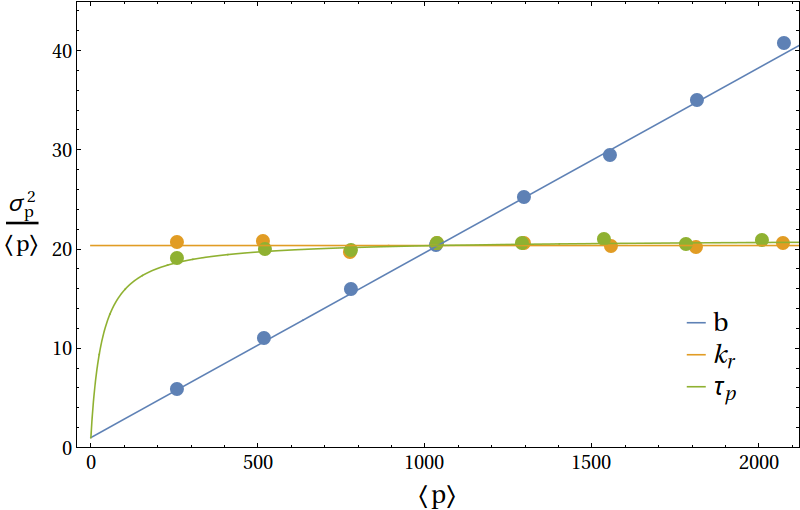
\includegraphics[width=11cm]{mas-sim_simple}
  \caption[Noise in proteins: comparing analytical results and simulations]{\label{fig:mas-sim_simple} Comparison between the results of the simulations (dots) and the analytical results (lines) given by eq. \eqref{eq:noise2}. The Fano factor is plotted vs. the mean. The legend indicates which parameter is varied while the others are fixed.}
\end{figure}

Therefore, the noise and the steady state average can be controlled independently by controlling the burst size $b$. If a cell produces many mRNAs and a few proteins per transcript (small $b$), the noise is reduced. On the contrary, the same average number of proteins can be reached by producing a few mRNAs and many proteins per mRNA (large $b$). In this case the noise is larger. Nevertheless there is an additional factor, reducing noise in this case requires a constant synthesis and degradation of mRNA. This is inefficient for the cells since they are inverting energy in the production of mRNAs from which there will be little proteins translated, representing a disadvantage in fitness. 

This analysis suggests that there is a pay-off between fitness and noise reduction in the cells that has been tuned by evolution according to the necessity of reliability of the particular genetic component. However, we will see that there are other mechanisms, like negative autorregulation, that allow cells to reduce noise in a more efficient way (see sec. \ref{sec:mas-neg_autorreg}).

\section{Several species with linear interactions}

In this section we generalize the previous results to arbitrary genetic network in which the interactions between its components are linear. To introduce the model, consider eqs. \eqref{eq:mas-simple_det_1} and \eqref{eq:mas-simple_det_2}. In matrix notation, they can be written as

\begin{equation}
  \label{eq:matdet}
  \mathbf{\dot{n}} = \left( \mathbf{A} - \mathbf{\Gamma} \right) \mathbf{n},
\end{equation}

where $\mathbf{n}^T=(d,n_1,n_2)$ is the vector of chemical species and the matrices $\mathbf{A}$ and $\mathbf{\Gamma}$ are defined as

\begin{align}
  \mathbf{A} &=
  \begin{pmatrix}
    0 & 0 & 0 \\
    k_r & 0 & 0 \\
    0 & k_p & 0
  \end{pmatrix} \label{eq:mas_A_single},\\
  \mathbf{\Gamma} &=
  \begin{pmatrix}
    0 & 0 & 0 \\
    0 & \gamma_r & 0 \\
    0 & 0 & \gamma_p 
  \end{pmatrix} \label{eq:mas_G_single}. 
\end{align}

Hence, $\mathbf{A}$ contains the creation rates and represents how each rate depends on the different species and $\mathbf{\Gamma}$ has the degradation rates, which is diagonal whenever the degradation is not mediated by interactions with other molecules.

Now, for an arbitrary circuit with an arbitrary number $N$ of species and linear interaction between them, we can write its deterministic equations in the form of eq. \eqref{eq:matdet}. Also, the state state space will have $N$ dimensions in the general case (see fig. \ref{fig:mas-trans_many}).

\begin{figure}[H]
  \centering
  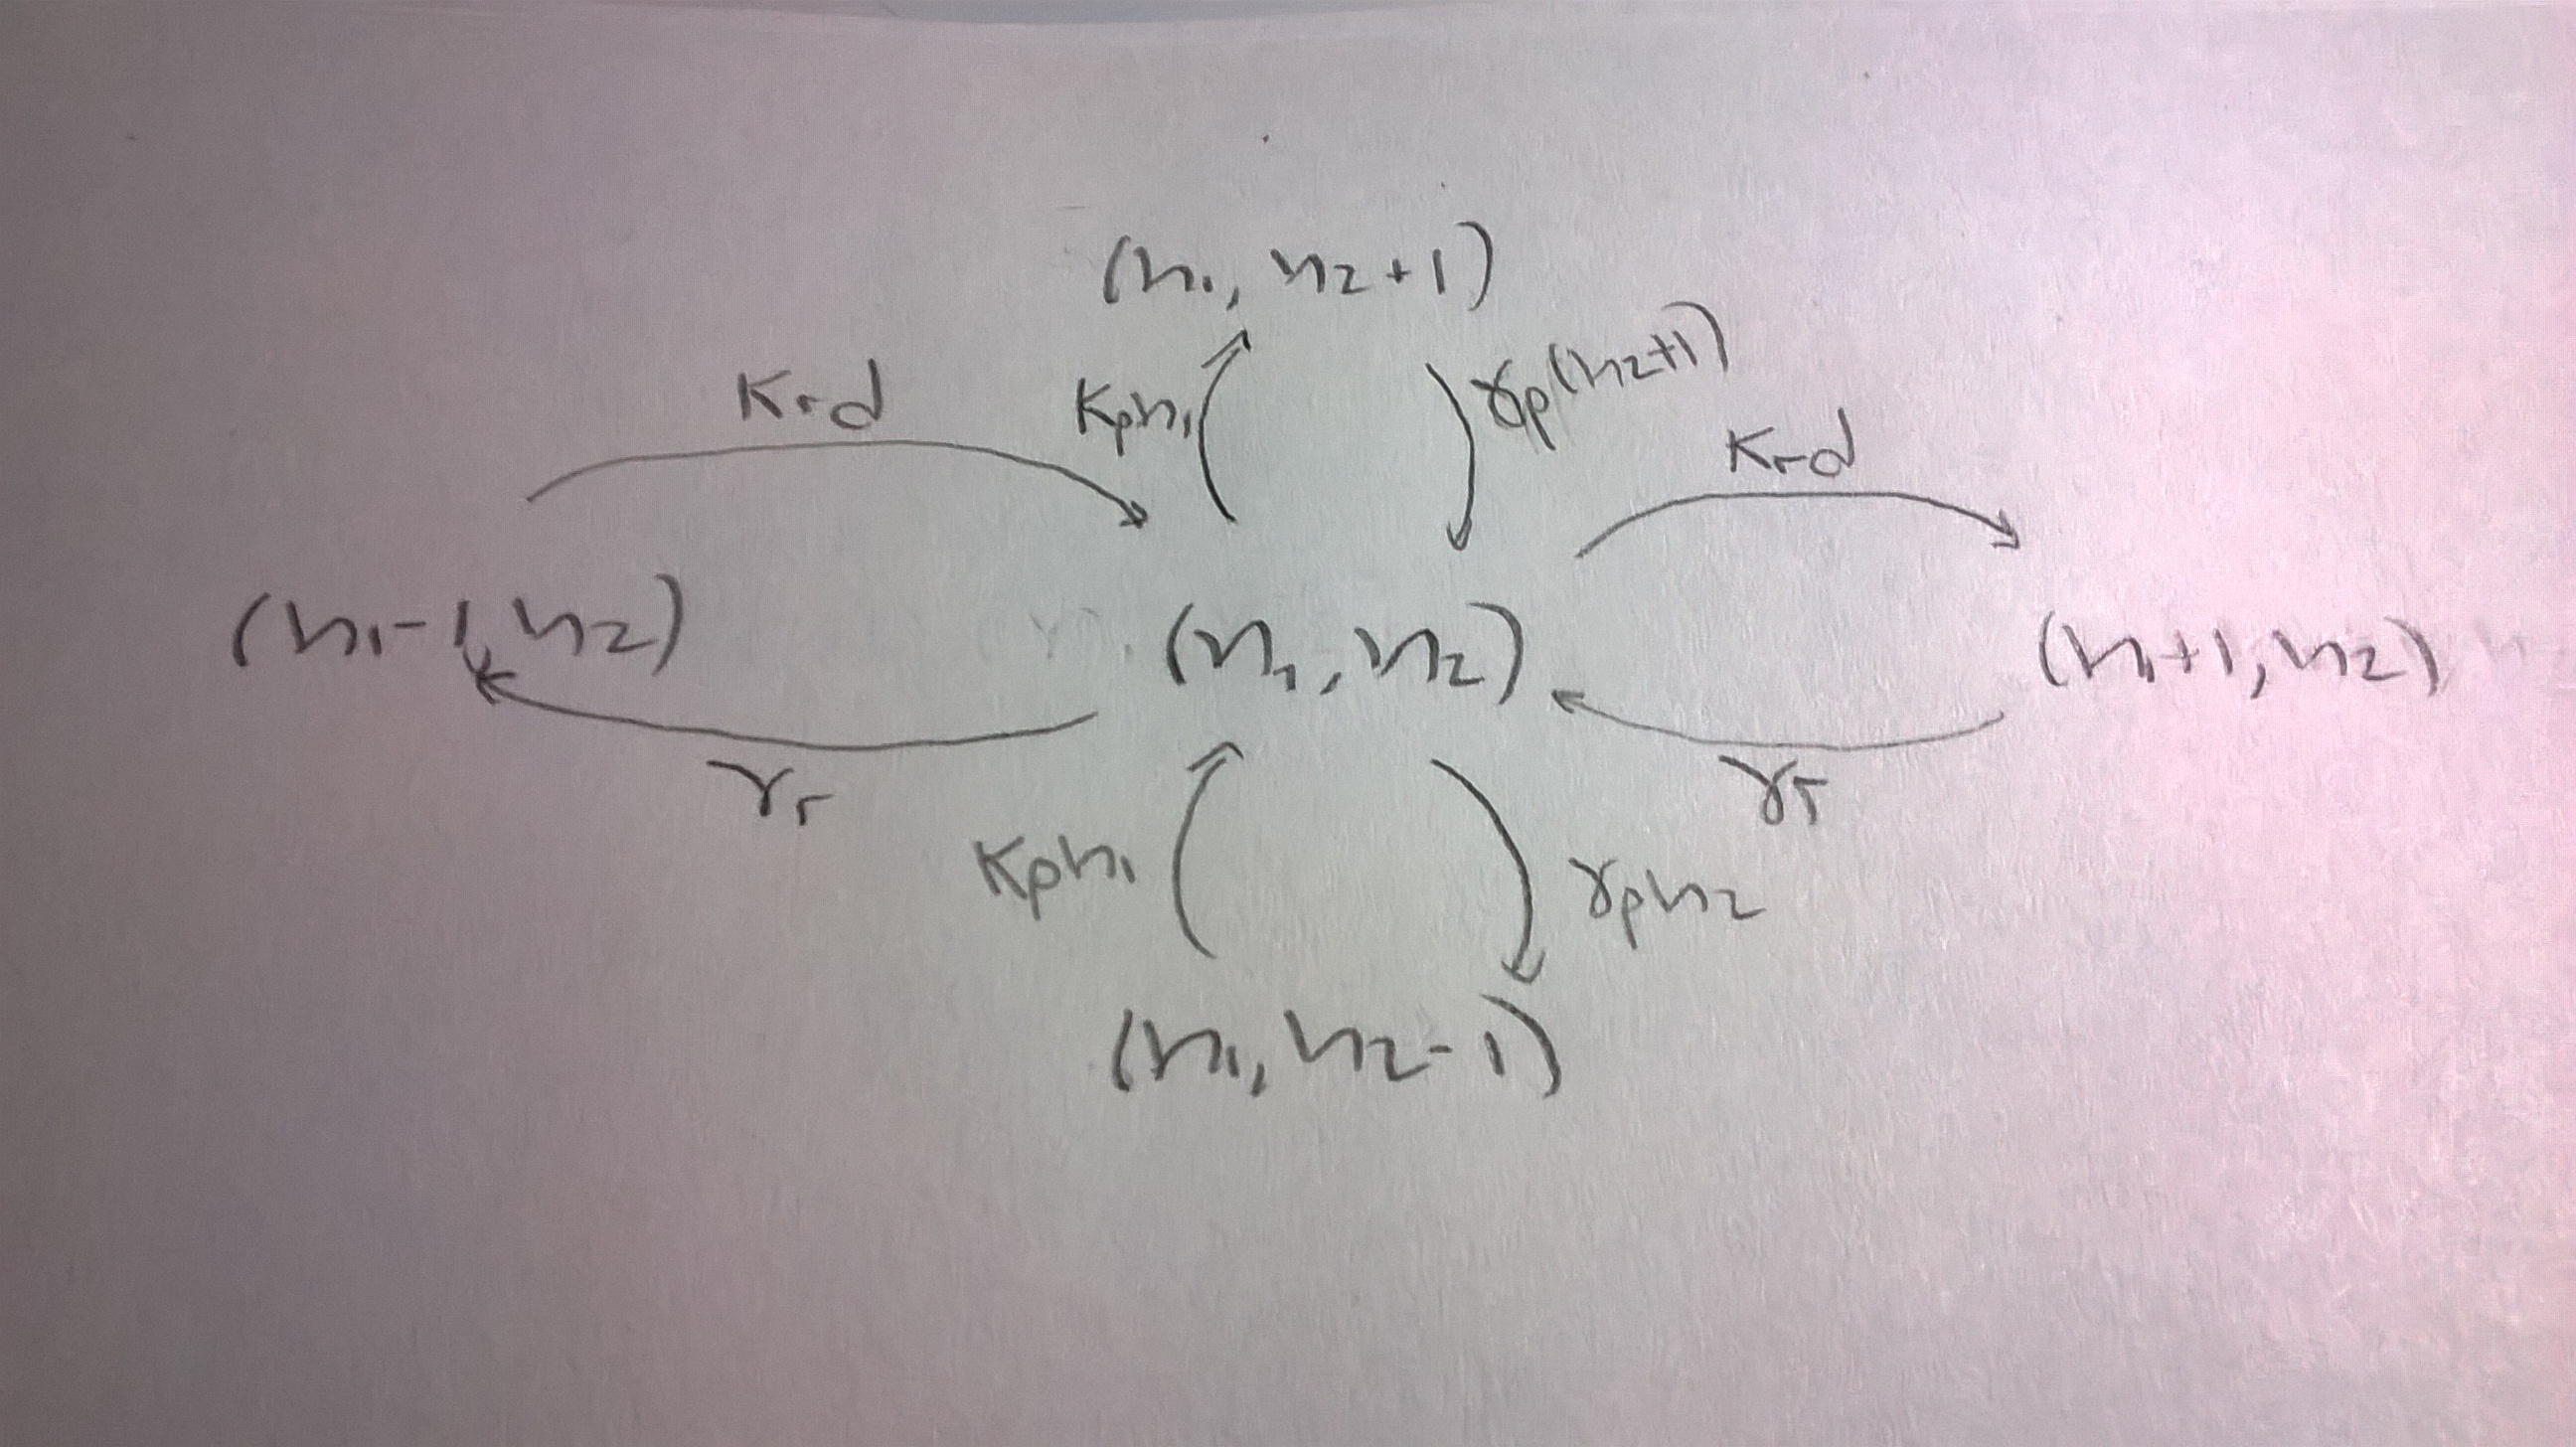
\includegraphics[width=9cm]{mas-trans_many}
  \caption[Transitions between states in general] {\label{fig:mas-trans_many} Scheme of the possible transitions in the case of three species.}
\end{figure}

According to fig. \ref{fig:mas-trans_many}, in the general case the master equation will have as many terms as there are transitions involving the state $\mathbf{n}$. The master equation can thus be written in general as follows

\begin{equation}
\label{eq:masterg1}
\dot{p}(n_i) =  \sum_{i=1}^N\left(\sum_{j=1}^N A_{ij}n_j \left( p(n_i-1) - p(n_i) \right) + \sum_{j=1}^N \Gamma_{ij}((n_j+1)p(n_i+1)-n_jp(n_i))\right)
\end{equation}

When for a fixed specie $i$, the terms in parentheses represent having $n_i-1$ molecules of the $i$th type and creating one; having $n_i$ and creating one; having $n_i+1$ and destroying one; and having $n_i$ and destroying one, respectively. Since this is possible for each of the $N$ types of molecules, we must sum over $i$ as well.

Assuming that degradation does not involve interactions between various molecules, the matrix $\Gamma$ can be taken to be diagonal, i.e. $\Gamma_{ij}=\delta_{ij}\Gamma_j$. With this eq. \eqref{eq:masterg1} becomes \footnote{To reduce the complexity of the expressions, we define $p(n_i) \coloneqq p(\mathbf{n}) = p(n_1,\dotsc,n_i,\dotsc,n_N)$, and $p(n_i\pm1)\coloneqq p(n_1,\dotsc,n_i\pm1,\dotsc,n_N)$. The same convention will be used for $F(z_i)$.}

\begin{equation}
\label{eq:masterg2}
\dot{p}(n_i) =  \sum_{i=1}^N\left(\sum_{j=1}^N A_{ij}n_j \left( p(n_i-1) - p(n_i) \right) + \Gamma_{i}((n_i+1)p(n_i+1)-n_ip(n_i))\right).
\end{equation}

We will follow the same procedure of the previous section, i.e. write the master equation in terms of the moment generating function and use its properties to find expressions for the moments. To get an equation for the moment generating functions, we multiply by $z_1^{n_1}\dotsm z_N^{n_N}$ and sum over $n_1,\dotsc n_N$, all from $0$ to $\infty$. At first, we will consider the term in parentheses of eq. \eqref{eq:masterg2} and later we will sum over $i$. For the first term we obtain the following expression \footnote{Again, to avoid having unnecesarily long expressions, we write $\sum$ refering to $\sum_{n_1=0}^\infty\dotsi\sum_{n_N=0}^\infty$.}

\begin{equation}
  \label{eq:momg1}
  \sum n_j z_1^{n_1}\dotsm z_i^{n_i}\dotsm z_j^{n_j}\dotsm z_N^{n_N} f(n_i) = z_iz_j\sum n_jz_j^{n_j-1}z_i^{n_i}f(n_i) = z_iz_j\frac{\partial F}{\partial z_j}. 
\end{equation} 

Where the same trick done previously to change indexes was used. Similarly, for the second term

\begin{equation}
  \label{eq:momg2}
  \sum n_jz_j^{n_j}z_i^{n_i}f(n_i) = z_j\frac{\partial F}{\partial z_j}.
\end{equation}

For the third and fourth terms

\begin{equation}
  \label{eq:momg3}
  \sum (n_i+1)z_i^{n_i}f(n_i+1) = \sum n_i z_i^{n_i-1}f(n_i) = \frac{\partial F}{\partial z_i}.
\end{equation}

\begin{equation}
  \label{eq:momg4}
  \sum n_iz_i^{n_i}f(n_i) = z_i\frac{\partial F}{\partial z_i}.
\end{equation}

Replacing eqs. \eqref{eq:momg1} - \eqref{eq:momg4} in eq. \eqref{eq:masterg2} we obtain the equation for the moment generating function

\begin{equation}
\dot{F}(z_i) = \sum_i\left( z_i\sum_jA_{ij}\frac{\partial F}{\partial z_j} - \sum_jA_{ij} z_j \frac{\partial F}{\partial z_j} + \Gamma_i\frac{\partial F}{\partial z_i} - \Gamma_iz_i\frac{\partial F}{\partial z_i}\right),
\end{equation}

which after factoring becomes

\begin{equation}
\label{eq:momg}
\dot{F}(z_i) = \sum_i(z_i-1)\left(\sum_jA_{ij} z_j \frac{\partial F}{\partial z_j} - \Gamma_i\frac{\partial F}{\partial z_i}\right).
\end{equation}

We have to differentiate it and use the properties \eqref{eq:con-mom_gen_d1} - \eqref{eq:con-mom_gen_d1d1} to obtain equations for the moments. Differentiating with respect to $z_l$

\begin{equation*}
\begin{split}
\frac{\partial \dot{F}}{\partial z_l} &= \sum_i\left[(z_i-1)\left[\sum_jA_{ij}\left(\delta_{jl}\frac{\partial F}{\partial z_j}+z_j\frac{\partial^2 F}{\partial z_j\partial z_l}\right)-\Gamma_i\frac{\partial^2 F}{\partial z_i\partial z_l}\right]\right.\\
&+\left.\delta_{il}\left(\sum_jA_{ij}z_j\frac{\partial F}{\partial z_j}-\Gamma_i\frac{\partial F}{\partial z_i}\right)\right].
\end{split}
\end{equation*}

\begin{equation*}
\begin{split}
\frac{\partial \dot{F}}{\partial z_l} &= \sum_i(z_i-1)\left[A_{il}\frac{\partial F}{\partial z_l}+\sum_jA_{ij}z_j\frac{\partial^2 F}{\partial z_j\partial z_l}-\Gamma_i\frac{\partial^2 F}{\partial z_i\partial z_l}\right]\\
&+\sum_jA_{lj}z_j\frac{\partial F}{\partial z_j}-\Gamma_l\frac{\partial F}{\partial z_l}.
\end{split}
\end{equation*}

Evaluating in $z_i=1$, $i=1,\dotsc,N$ we otain after applying the properties of $F$

\begin{equation*}
\dot{\langle n_l \rangle} = \sum_jA_{lj}\langle n_j\rangle-\Gamma_l\langle n_l\rangle,
\end{equation*}

and writing in matrix form

\begin{equation}
  \label{eq:mas-general_ave}
  \dot{\langle \mathbf{n}\rangle} = (\mathbf{A}-\mathbf{\Gamma})\langle \mathbf{n}\rangle.
\end{equation}

Which has the form of eq. \eqref{eq:matdet}, but for the averages as expected. Now differentiating again with respect to $z_m$ and doing some algebra

\begin{equation*}
  \begin{split}
    \frac{\partial^2 \dot{F}}{\partial z_l \partial z_m} &= \sum_i(z_i-1) \left(A_{im}\frac{\partial^2F}{\partial z_i \partial z_m} + \sum_jA_{ij}z_j\frac{\partial^3F}{\partial z_j \partial z_l \partial z_m}+A_{il}\frac{\partial^2F}{\partial z_l\partial z_m} - \Gamma_i\frac{\partial^3F}{\partial z_i \partial z_l \partial z_m}   \right)\\
    &+\sum_jA_{mj}z_j\frac{\partial^2F}{\partial z_j\partial z_l}+A_{ml}\frac{\partial F}{\partial z_l} - \Gamma_m\frac{\partial^2F}{\partial z_l\partial z_m}\\
    &+ A_{lm}\frac{\partial F}{\partial z_m} + \sum_jA_{lj}z_j\frac{\partial^2F}{\partial z_j\partial z_m}-\Gamma_l\frac{\partial^2F}{\partial z_l\partial z_m}.
  \end{split}
\end{equation*}

Evaluating at $z_i=1$ for all $i$ we obtain

\begin{equation*}
  \frac{\partial^2\dot{F}}{\partial z_l \partial z_m} = \sum_jA_{mj}z_j\frac{\partial^2F}{\partial z_j\partial z_l}+A_{ml}\frac{\partial F}{\partial z_l} - \Gamma_m\frac{\partial^2F}{\partial z_l\partial z_m} + A_{lm}\frac{\partial F}{\partial z_m} + \sum_jA_{lj}z_j\frac{\partial^2F}{\partial z_j\partial z_m}-\Gamma_l\frac{\partial^2F}{\partial z_l\partial z_m}.
\end{equation*}

Which can be rewritten as

\begin{equation*}
  \begin{split}
    \frac{\partial^2\dot{F}}{\partial z_l \partial z_m} &= \sum_j\left(A_{mj}z_j-\Gamma_{mj}\right)\frac{\partial^2F}{\partial z_j\partial z_l} + \sum_jA_{mj}\delta_{jl}\frac{\partial F}{\partial z_j}\\
    &+\sum_j\left(A_{lj}z_j-\Gamma_{lj}\right)\frac{\partial^2F}{\partial z_j\partial z_m} + \sum_jA_{lj}\delta_{jm}\frac{\partial F}{\partial z_j}.
  \end{split}
\end{equation*}

Which is valid for all $l$ and $m$, evaluating at $z_i=1$ for all $i$ we get after writing in matrix form

\begin{equation}
  \label{eq:mas-general}
  \boxed{\nabla\nabla^T\dot{F}|_1 = \left(\left(\mathbf{\Gamma} - \mathbf{A}\right)\nabla\nabla^TF|_1 - \mathbf{A}\mathbf{\Theta} F|_1\right)+\left(\left(\mathbf{\Gamma} - \mathbf{A}\right)\nabla\nabla^TF|_1 - \mathbf{A}\mathbf{\Theta} F|_1\right)^T}
\end{equation}

\todo[inline]{Do I have to include more steps? or to explain the expression with more detail?}

Where $\Theta_{ij} \coloneqq \delta_{ij}\frac{\partial}{\partial z_i}$. The set of linear equations can be solved for the moments and correlation using a computer program. Therefore, given the specific form of the matrices $\mathbf{A}$ and $\mathbf{\Gamma}$, we only have to replace on eq. \eqref{eq:mas-general_ave} and \eqref{eq:mas-general} to find the moments and the noise. In the next section we will apply them to a particular case.

\section{Several species with non-linear interactions - Negative autorregulation}
\label{sec:mas-neg_autorreg}

As we have seen on sec. \ref{sec:hill}, the interactions between the component of a genetic circuits are non-linear. As a consequence, there might be several fixed points. To use this approach we need to identify the stable fixed points, linearize about each of them, each linearization yields to a pair of matrices $\mathbf{A}$ and $\mathbf{\Gamma}$ and we solve for each of them eqs. \eqref{eq:mas-general_ave} and \eqref{eq:mas-general}.

We will consider the case of negative autorregulation, in this case $k_r$ is now a Hill function for a repressor (eq. \eqref{eq:con-hillac}) that depends on the number of proteins of the same gene, taking the case with no basal transcription rate, the deterministic equations are

\begin{align*}
  \dot{n_1}(t) &= \frac{k_r^{\text{max}}}{1+\left(\frac{n_2(t)}{K_d}\right)^n}d - \gamma_rn_1(t),\\
  \dot{n_2}(t) &= k_pn_1(t)-\gamma_pn_2(t).
\end{align*}

\todo[inline]{Include histogram and plot of Hill function to explain qualitatively why does it reduces noise, average and has only one fixed point}

Making a first order Taylor expansion of $k_r$ about its value at the steady state we get

\todo[inline]{Recall the machete que ellos meten ahi, d must be constant}

\begin{equation}
  \begin{split}
  k_r(n_2) &\approx k_r(\langle n_2\rangle_s) + \left.\frac{\mathrm{d}k_r(n_2)}{\mathrm{d}n_2}\right|_{\langle n_2\rangle_s}\left(n_2-\langle n_2\rangle_s\right)\\
  &=\frac{k_r^{\text{max}}}{1+\left(\frac{\langle n_2\rangle_s}{K_d}\right)^n} - \frac{k_r^{\text{max}}n\left(\frac{\langle n_2\rangle_s}{K_d}\right)^{n-1}}{K_d\left(1+\left(\frac{\langle n_2\rangle_s}{K_d}\right)^n\right)^2}\left(n_2-\langle n_2\rangle_s\right)\\
  &= k_0-\frac{k_1}{d}n_2,
  \end{split}
\end{equation} 

where $k_0$ and $k_1$ are given by

\begin{equation*}
  k_0\coloneqq k_r(\langle n_2\rangle_s) - \left.\frac{\mathrm{d}k_r(n_2)}{\mathrm{d}n_2}\right|_{\langle n_2\rangle_s}\langle n_2\rangle_s,\quad\quad k_1 \coloneqq -\left.\frac{\mathrm{d}k_r(n_2)}{\mathrm{d}n_2}\right|_{\langle n_2\rangle_s}n_2. 
\end{equation*}

Therefore, the matrix $\mathbf{A}$ becomes

\begin{equation*}
  \mathbf{A} =
  \begin{pmatrix}
    0 & 0 & 0 \\
    k_0 & 0 & -k_1 \\
    0 & k_p & 0
  \end{pmatrix}
\end{equation*}

and $\mathbf{\Gamma}$ is the same as in \eqref{eq:mas_G_single}. Solving eqs. \eqref{eq:mas-general_ave} and \eqref{eq:mas-general} we get

\begin{equation}
  \label{eq:mas-autorreg_final}
  \boxed{\langle n_2\rangle_s = \frac{1}{1+b\phi}\frac{k_0b}{\gamma_p}},\quad\quad \boxed{\nu_2 = \frac{1-\phi}{1+b\phi}\frac{b}{1+\frac{\gamma_p}{\gamma_r}}+1},
\end{equation}

\todo[inline]{Specify more about the solution?}

with $\phi\coloneqq k_1/\gamma_p$ representing the strength of the feedback. In figure \ref{fig:mas-sim_autorreg}, we compare eq. \eqref{eq:mas-autorreg_final}  with a Gillespie simulation using the exact rates. Altought the analytic expressions are approximate, there is an excellent match with the simulations.

\begin{figure}[H]
  \centering
  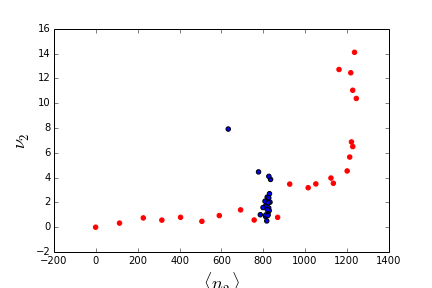
\includegraphics[width=11cm]{mas-sim_autorreg}
  \caption[Autorregulation simulation results]{\label{fig:mas-sim_autorreg} Fano factor vs. average number of proteins. The solid lines correspond to eq \eqref{eq:mas-autorreg_final}, while the point represent the Gillespie simulations. In the blue part $n$ was varied and in the orange $K_d$ was varied.}
\end{figure}

\section{Final remarks and further applications}

\todo[inline]{Write this section}
